\documentclass{project}
\usepackage[pdfauthor={C. P. Marriott},pdftitle={Software Engineering Group Project, Project Plan},pdftex]{hyperref}
\usepackage[pdftex]{graphicx}
\usepackage{pdfpages}
\hypersetup{colorlinks=false,pdfborder={0 0 0}}
\begin{document}
\title{Software Development Life cycle}
\subtitle{Design Specification}
\author{Tom Reed, Matt Whitmore, Dave Clark, Silhab Csoma, Mike Steel, Chris 'Tux' Lloyd, Aleksandra Badyda, Samuel Jackson, Chris Marriott}
\shorttitle{Design Specification}
\version{1.3}
\status{draft}
\date{2012-12-5}
\configref{SE.17.DS.01}
\maketitle
\tableofcontents
\newpage
\section{Introduction}
\subsection{Purpose of this Document}
This should provide everything designers, programmers and testers need to know to use the facilities
provided by a module. It should include an outline for all parts of the system. The information provide should be enough to get a basic understanding of the system.

\subsection{Scope}
An outline for each class and its containing methods. Explanation of how the server works and significant algorithms. Outline of how the system is navigated and operated through sequence diagrams.

\subsection{Objectives}
The objective of this document is to give an overview of the system that is being produced.
\\
The areas covered by this plan are:
\begin{itemize}
	\item Java Classes explanations
	\item Sequence diagrams
	\item Relational Database diagram
	\item JSON Table
	\item Algorithms
\end{itemize}

\section{General Functionality}
\subsection{Description}
An HTTP servlet is used to access the data contained within the backend of the server as if it was almost a web page.  We will pass parameters between it and get a response. We will be working on the principle that one main servlet will perform different actions, passing through an actions variable and any data required to be processed. There are two methods of accessing this; using ‘get’ and ‘post’ requests.  The get request will pass the parameters through the URL, the post request through a hidden layer, based on the users input. JavaScript will collate the necessary data, and attach the appropriate action command before sending to the server.
\subsection{Relational Database diagram}
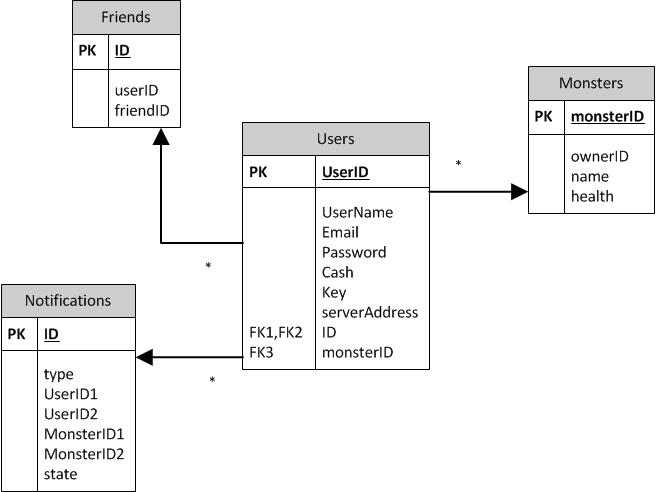
\includegraphics{relationshipDiagram.jpg}
\subsection{Relational Database diagram explanation}
This is a relational database diagram for our database, we have used 4 tables to store information about the User, the Users table to store information directly related e.g. user name etc.  We then have the Monsters table in which will have information about the user’s monsters, the friends table to store the user’s friends and the notifications table to store information about any notification the user might have e.g. a user who wants to battle their monster with you.

\section{Algorithms}
The algorithm for the aging process ind strengths as follows:\\
=(10+2.7*A)*EXP((A*(-0.09)))\\
The A is the number of days that have passed. Upon birth it is at 100\% health, after 7 days it rises to 150\%. After 21 days(3 weeks) it's back to 100\% and at 84 days(12 weeks) the monster shall be at 0\%(Dead). 

\section{JSON Table}
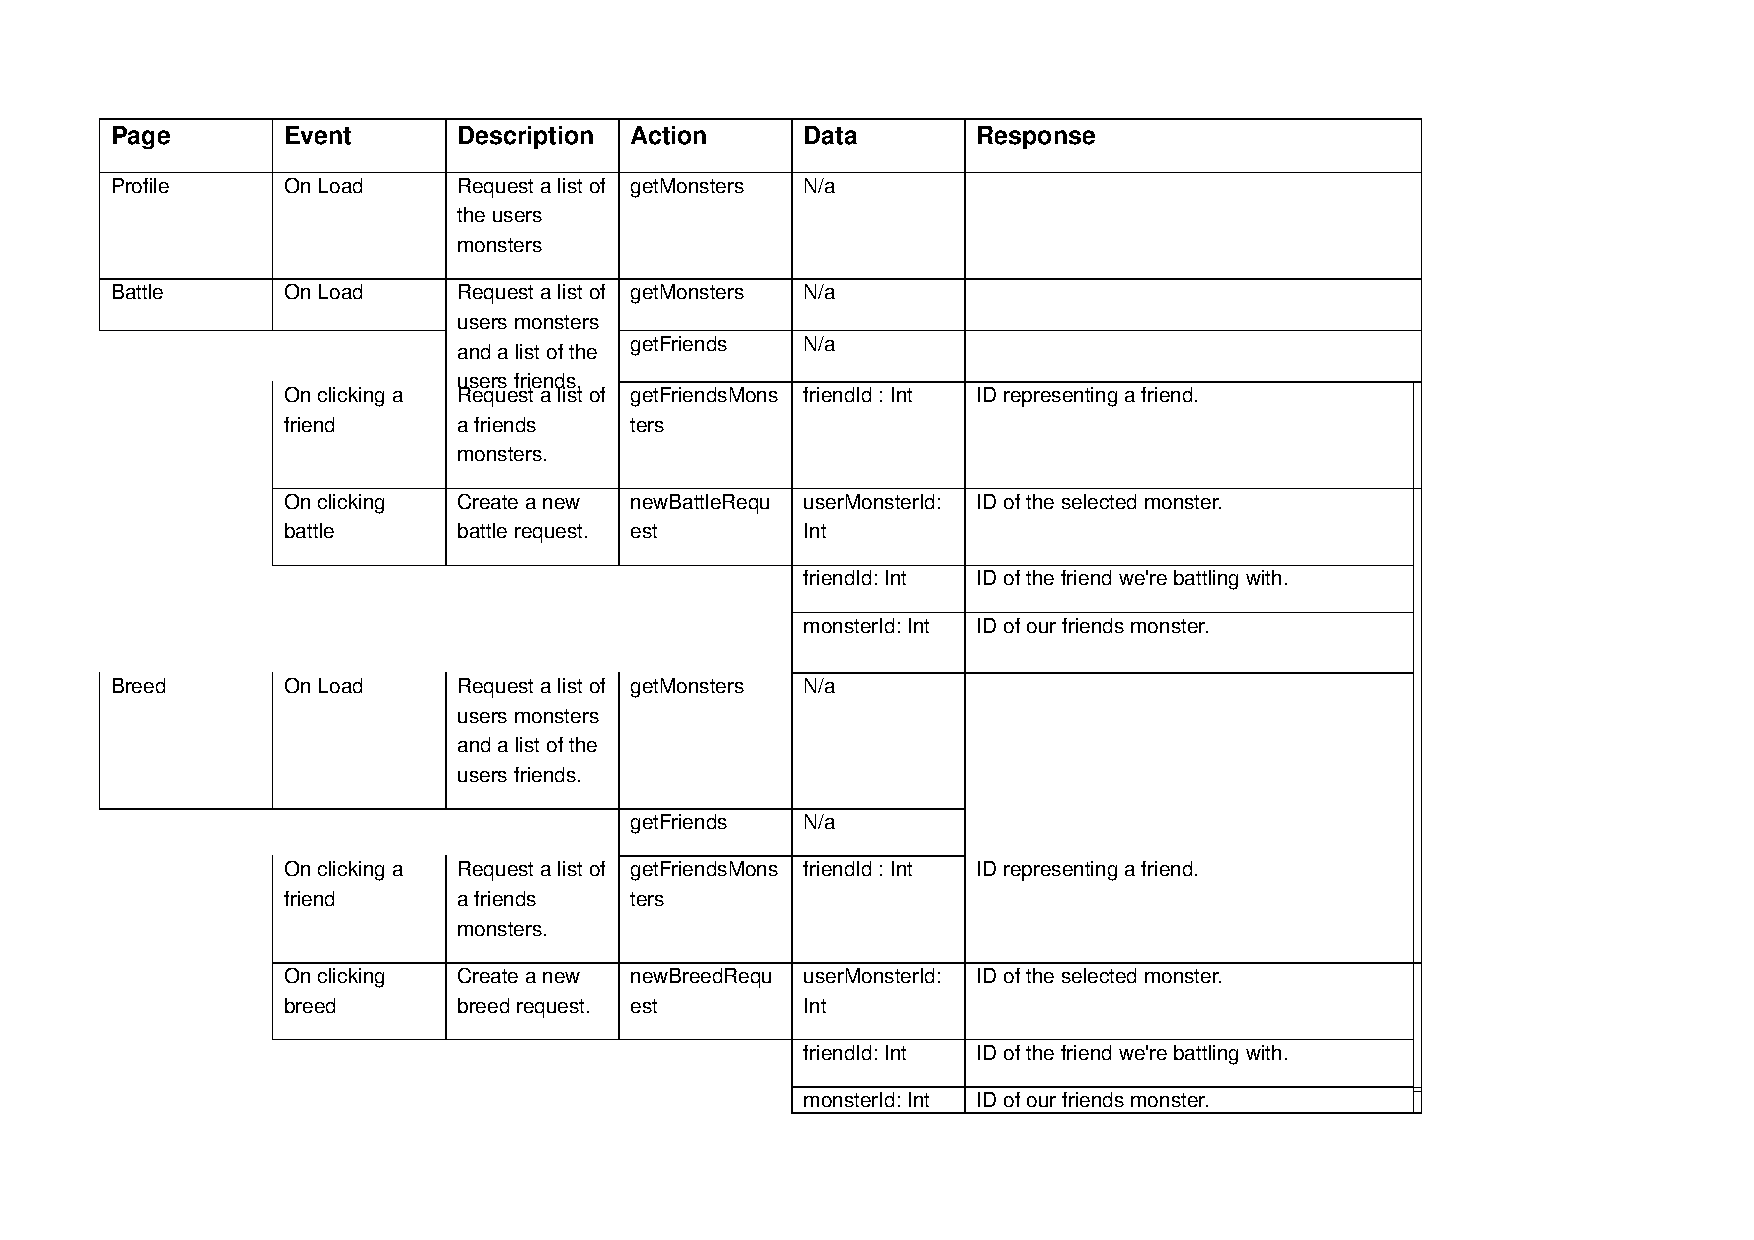
\includepdf[pages={1-2}]{Requests.pdf}

\subsection{JSON Explanation}
JSON (also known as JavaScript Object Notation) is a form of data interchange that is designed to be "human readable". Derived from the JavaScript scripting language, it shows simple data structures and associative arrays, which they call "objects". This table shows us the various data interchanges that take place within the design of our project.  JSON is used as an alternative to XML.

\section{Class Diagram}
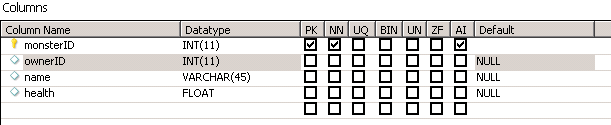
\includegraphics[scale=0.40]{MonsterDiagram.png}

\section{Significant Data Classes}
\subsection{Java Data Classes}
There are four main classes within the Java designed to be implemented within the project, these are Monster, User, User-Manager, and Request.
\subsection{User-Manager class}
User-Manager handles the basic ability to get a user from the database and find out if they exist, as well as being able to add and remove a user from the database. This class is therefore key to having a usable log in page, as well as being absolutely necessary for a functioning registration form for new users.
\subsection{User class}
The User class handles more specific details appropriate to a user, including both details necessary for the user logging in, such as getting the user-name and password, as well as details necessary for the management of the user within the game, such as methods to get which monsters the user has. There will also be parts of this class that handle setting the user-name and password and other key parts of the user’s details, so this is a class key to many functions of the website; from creating a new user and logging in, to finding out what monsters and friends that user has.
\subsection{Monster class}
There is then the Monster class which will handle all the functionality regarding monsters that a user might own, including basic things such as who owns the monster, its stats, and what its name is, to key details that add depth to the game, such as the monster’s age, how many battles it has won, and how fertile it is.
\subsection{Request class}
Finally, there is the Request class, which will handle requests from other players to breed, fight, or become friends. This will handle everything to do with notifying the recipient of these requests, such as noting who the request is from, and responding to it.

\subsection{Functional Requirements}
\begin{table}[!h]
\centering
\begin{tabular}{|l|c|r}
\hline
Monster & FR3, FR4, FR10 \\ \hline
User & FR1, FR6, FR7, FR8, F11 \\ \hline
User-Manager & FR1, FR2, FR3, FR7 \\ \hline
Request & FR6, FR9 \\ \hline
\end{tabular}
\caption{This table shows the functional of Java classes}
\label{tab:myfirsttable}
\end{table} 

\section{Breed Class}
The breed class is called Breed.class and is a private class.
\subsection{Public Methods} 
The only public method this class has is ENUM Breed and has no parameters. This is a list of set monster types that the monster will be of type. Used ENUM so can only select a type from that list.

\section{Monster Class}
The monster class is called Monster.class and is a public class.
\subsection{Public Methods}
This class contains getter and setters for monster attributes. The getters and setters are for id, ownerId, name, stats, breed, status, birth, cashPrize, wins and losses. They set the value and return the value for the monster.

\section{MySQLDatabase Class}
The MySQLDatabase class is called MySQLDatabase.class and is a public class.
\subsection{Public Methods}


\section{Request}
The Request class is called Request.class and is a public class.
\subsection{Public Methods}
public User getFrom() - This will return from which is of type User. public void setFrom(User from) - This will set the User from and take User from as a parameter.
public User getTo() - This will return to which is of type User. public void setTo(User to) - This will set the User to value and take User to as a parameter.
public Monster getFromMon() - This will return fromMon which is of type Monster. public void setFromMon(Monster fromMon) - This will set fromMon and takes Monster fromMon as a parameter.
public Monster getToMon() - This will return a toMon which is of type Monster. public void setToMon(Monster toMon) - This will set toMon and takes Monster toMon as a parameter.
public RequestType getType() - This will return type which is of type request. public void setType(RequestType type) - This will set type and take RequestType type as a parameter. These will be used to determine whether it is pending, accepted and declined.
public RequestState getState() - This will return state which is of type RequestState. public void setState(RequestState state) - This will set state which is of type RequestState and takes RequestState state as a parameter.

\section{Request state}
The request state class is called RequestState.class and is a public ENUM class.
\subsection{Public Methods}
The only method in this class is enum RequestState. This is used to allow 3 states to be identified of which are ACCEPTED, PENDING and DECLINED. These will be used for requests such as battle and breed.

\section{UserManager}
The user manager class is called UserManager.class and is a public class.
\subsection{Public Methods}
public UserManager() - 
public User fetchUser(Integer id)
public User getUser(String name)
public void addUser(User user)
public void removeUser(User user)
public void createUser(Integer id, String username, String email, String password)


\section{User}
The user class is called User.class and is a public class.
\subsection{Public Methods}
public Integer getId() - This will return id which is of type Integer. public void setId(Integer id) - This will set id and takes Integer id as a parameter.
public String getUsername() - This will return username which is of type String. public void setUsername(String username) - This will set username and takes String username as a parameter.
public Integer getKey() - This will return key and is of type Integer. public void setKey(Integer key) - This will set key and takes Ineger key as a parameter.
public String getEmail() - This will return email and is of type String. public void setEmail(String email) - This will set email and takes String email as a parameter.
public String getPassword() - This returns password and is of type String. public void setPassword(String password) - This will set the password and takes String password as a parameter.
public Integer getCash() - This will return cash and is of type Integer. public void setCash(Integer cash) - This sets cash and takes Integer cash as a parameter.
public String getServerAdd() - This will return serverAdd and is of type String. public void setServerAdd(String serverAdd) - This sets serverAdd and takes String serverAdd as a parameter.
public ArrayList\textless Monster\textgreater  getMonsters() - This will return a list of monsters of type ArrayList\textless Monster\textgreater. public void setMonsters(ArrayList\textless Monster\textgreater  monsters) - This sets monsters and takes ArrayList\textless Monsters\textgreater  monsters as a parameter.
public ArrayList\textless User\textgreater  getFriends() - This will return a list of friends of type ArrayList\textless User\textgreater. public void setFriends(ArrayList\textless User\textgreater  friends) - This sets friends and takes ArrayList\textless User\textgreater  friends as a parameter.
public ArrayList\textless Request\textgreater  getRequests() - This will get a list of requests of type ArrayList\textless Request\textgreater. public void setRequests(ArrayList\textless Request\textgreater  requests) - This will set requests and takes ArrayList\textless Request\textgreater  requests as a parameter.


\section{Status class}
The Status class is called Status.java and is a public enum class.
\subsection{Public methods}
This class is an ENUM class and defines a set of 4 statuses that monsters can have. NORMAL, SICK, DEAD and HAPPY.


\section{RequestType class}
The Request type class is called RequestType.class and is a public ENUM class.
\subsection{Public methods}
This class is an ENUM class and defines a set of 3 types for request. BATTLE, BREED and FRIEND. 

\section{Data Storage}
Within the java programing the data is stored in a number of ways, a major way that data will be handled is through enums; requests will be handled through this and will be stored as either battle, breed, or friend, and the states of these requests will also be stored as enums, being either accepted, viewing, pending, or declined. Also stored as enums will be the statuses of monsters, thusly each monster status will be handled as normal, sick, dead, or happy.  Breed considers the different types of monster that we plan to be breeding with each other, and this therefore will be stored as an enum with the value of slime, beast, demon, dragon, serpent, or ghost.

Array Lists will also be used, but only, as far as designed, in private instances, so there will be no public instances that need to be explained in class diagrams. Otherwise, usernames, passwords, and the like will be handled in private strings and variable types as are appropriate. 


\section{Sequence Diagrams}
\subsection{Accept Battle}
This sequence diagram shows a user accepting a battle request that has been sent to them by a friend. The diagram shows the users response being sent to the server using the “doPost” method. The request then runs through the relevant classes in order to gain the information required.
\begin{center}
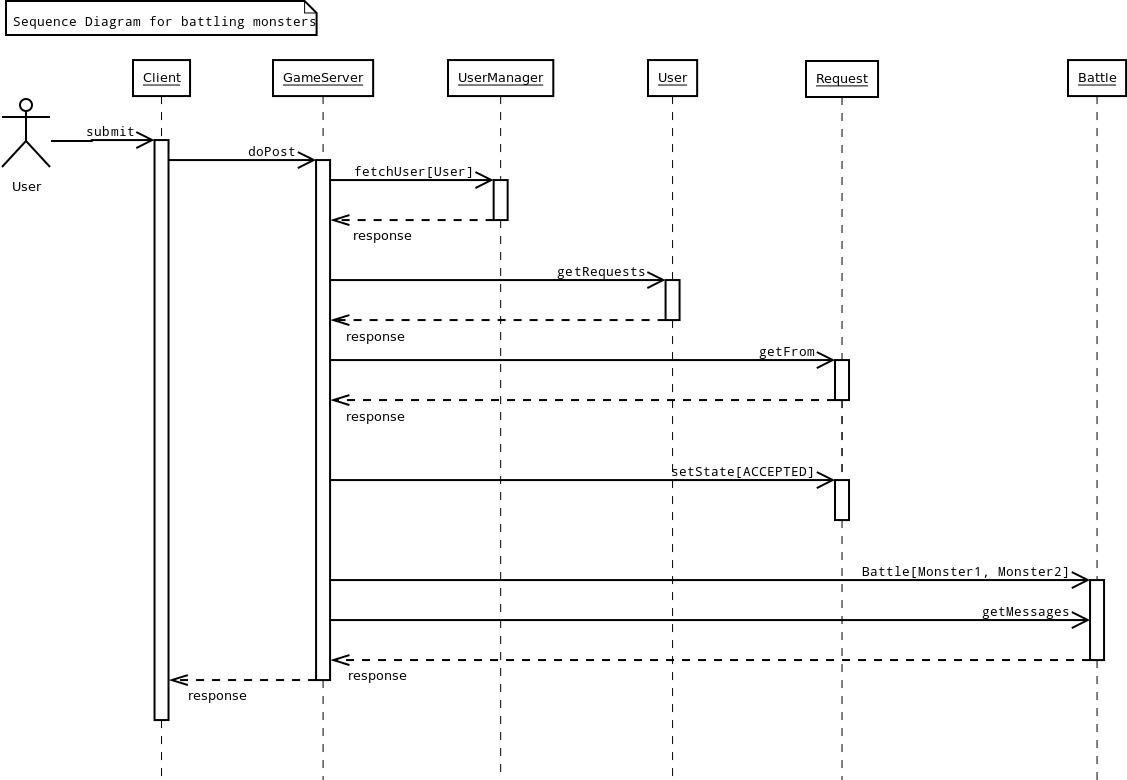
\includegraphics[scale=0.40]{SD_accept_battle.png}
\end{center}

\subsection{Accept Breed}
This sequence diagram shows a user accepting a breed request that has been sent to them by a friend. The diagram shows the users response being sent to the server using the “doPost” method. The request then runs through the relevant classes in order to gain the information required.
\begin{center}
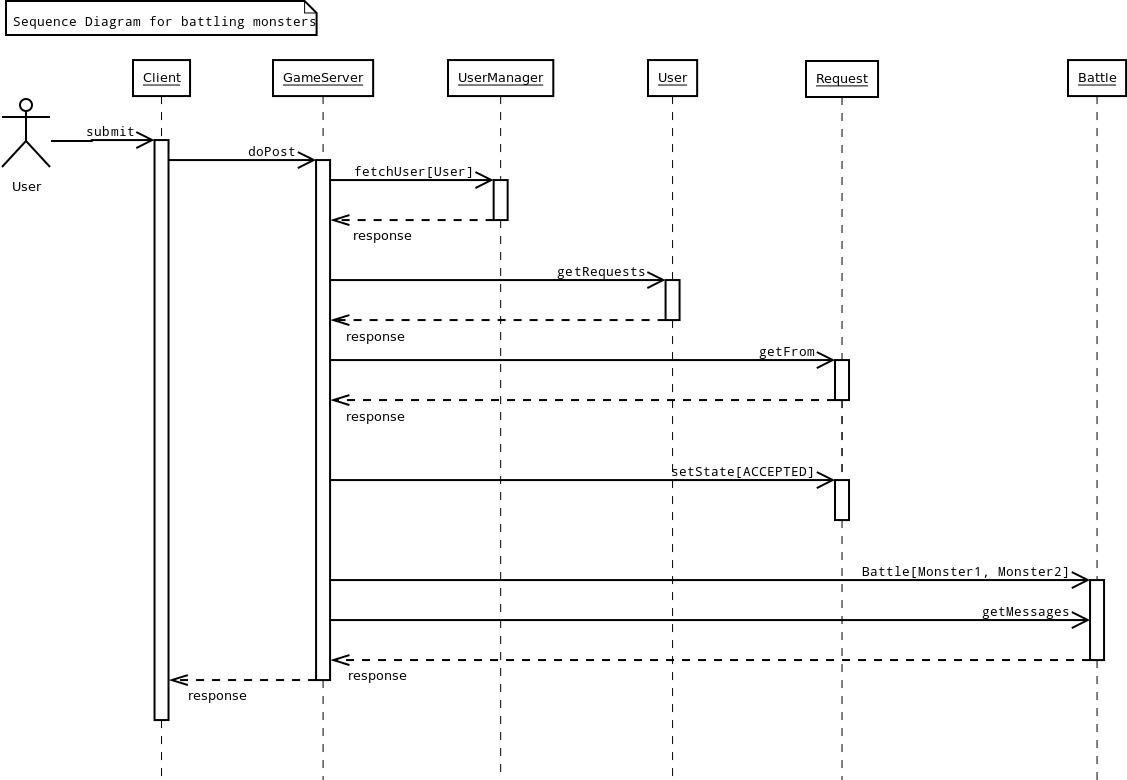
\includegraphics[scale=0.40]{SD_accept_breed.png}
\end{center}

\subsection{Add Friend}
This sequence diagram shows a user adding a friend. The users request is sent to the server using the “doPost” method. The request then runs through the relevant classes in order to gain the information required. A request is then sent to the corresponding user using the “addRequest” method and “User class”.
\begin{center}
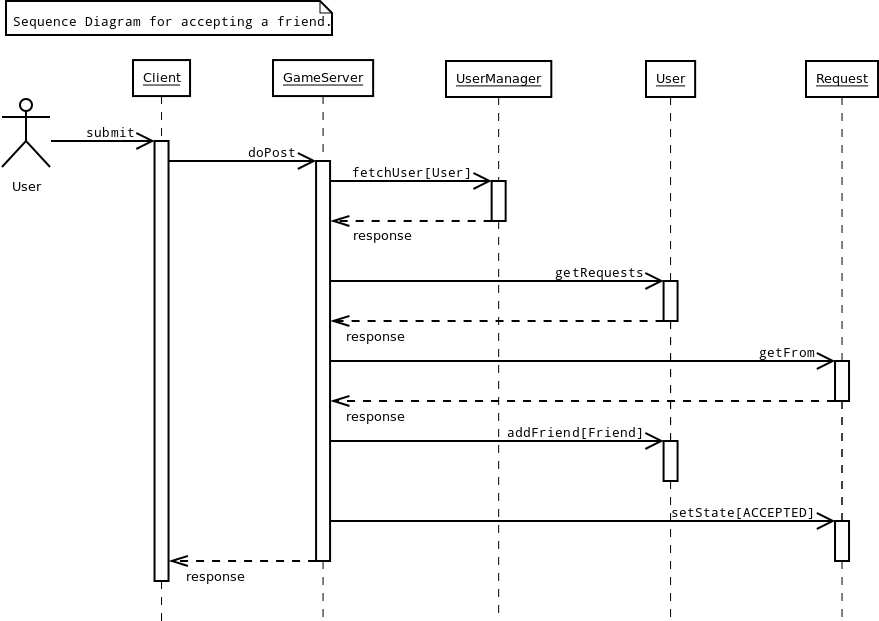
\includegraphics[scale=0.40]{SD_accept_friend.png}
\end{center}

\subsection{Register User}
This sequence diagram shows a user submitting their password and username to create a monstermash account. The diagram shows the users password and username being sent to the server using the “doPost” method. The request then runs through the relevant classes in order to process the users details and create the new account.
\begin{center}
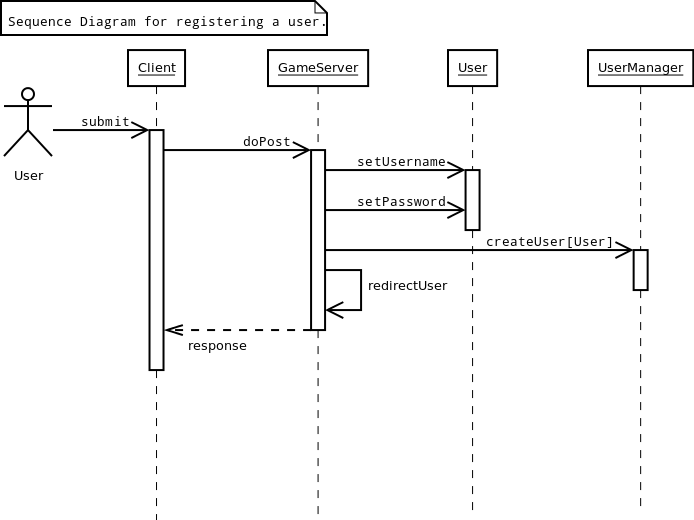
\includegraphics[scale=0.40]{SD_register_user.png}
\end{center}

\subsection{Send Battle/Breed Request}
This sequence diagram shows a user sending a breed or battle request to a friend. The diagram shows the users request being sent to the server using the “doPost” method. A request is then sent to the corresponding user using the “addRequest” method and “User class”.
\begin{center}
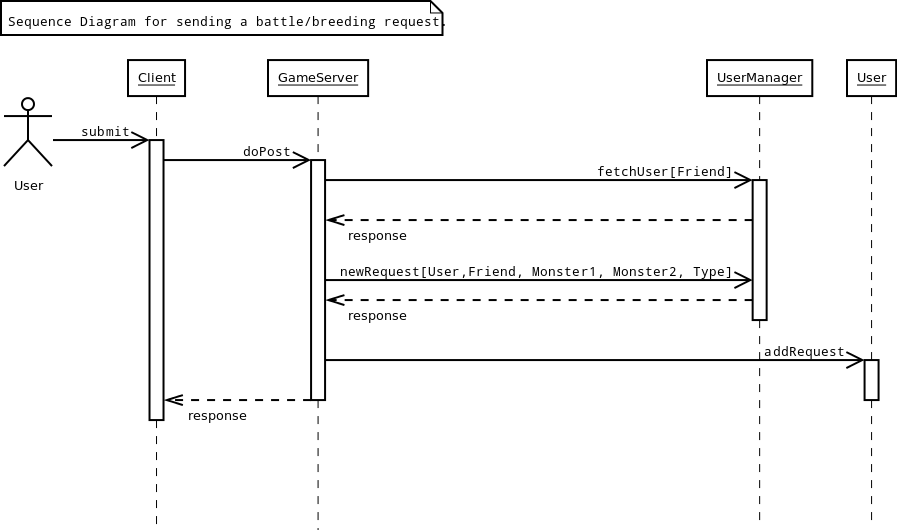
\includegraphics[scale=0.40]{SD_send_battle_breed_request.png}
\end{center}

\subsection{User Log In}
This sequence diagram shows a user logging in to monstermash. The user submits their login information and it is posted to the server using the “doPost” method. The request then runs the the relevant classes, checking the login details. A response is generated if the login details are invalid or the user is logged in if they details are valid.
\begin{center}
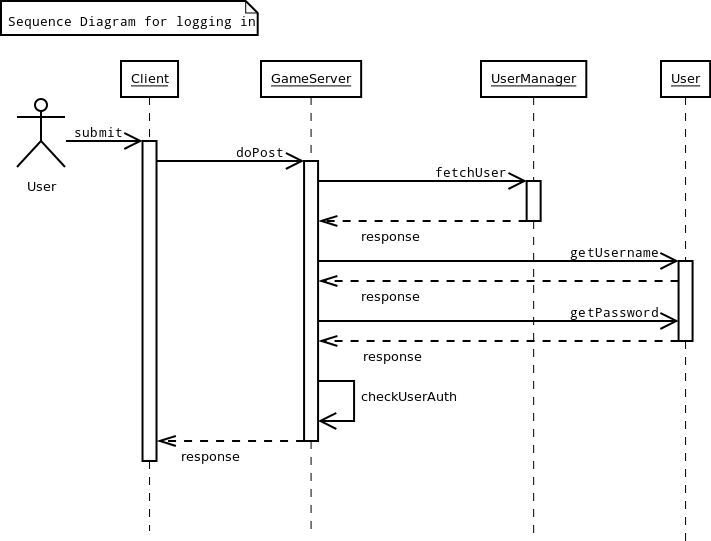
\includegraphics[scale=0.40]{SD_user_login.png}
\end{center}

\section{State Diagram}
\begin{center}
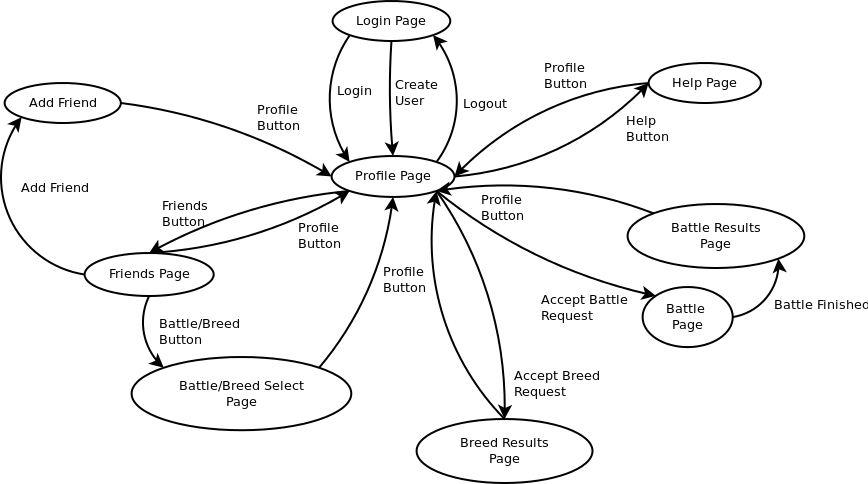
\includegraphics[scale=0.50]{state_diagram.png}
\end{center}

\subsection{State Diagram Description}

As you can see, the diagram above shows the design structure for how we want to be able to navigate each of our web pages. I will go through each connection individually, and explain the reasoning behind each.

\subsubsection{Login Page to Profile Page}

This is the first page that the user will be able to see when going onto our website, the page will require the user to enter their username and password into the allocated areas, once this is done, the user will be taken to the profile page, this is because the profile page is regarded as the users most important page, as this is where the user can decide what s/he plans to do.

\subsubsection{Profile page to Various pages}

The reason we had the profile page link to most of the pages on the website, was simply because this page acts almost as the “home” page of our structure, and it makes it easier for the user to have just one page in which they can select most of their options. If we separated and spread out each of the links to various pages to other pages in the structure, this would likely confuse and frustrate the user, by having them all in the same place, this avoids most issues about navigation that may arise.

\subsubsection{Profile page to Help page}

It is most likely that if the user had a problem, they would not be on any page other than the profile page, as this would be the starting point for the user, for this reason, we linked the “Help” page only too and from the profile page.

\subsubsection{Profile page to Battle page}

As the “Battle” page one of the most important pages (Alongside Friends) it was important that we put the link to this page in an obvious place, and there is no place more obvious than on your “Profile” page, as (as was explained before) this page works as the “home” page of this website, a page that is constantly referred to.

\subsubsection{Battle page to Battle results page}

After you have accepted an offer of a fight, the user will be taken to an area called the “Battle” page, in which you can watch the battle between your monster and the opponent that challenged you, after the battle has been completed you will be taken to the Battle results page, we structured this so that if you are the user that sent out the battle request, you will automatically be taken to the “Battle Results” page, as (as we have explained previously) the user sending out battle requests does not get to view the battle, but just see’s the results. After the users have seen the results of their battle(s), they have the option to return to the “Profile” page, so that they can continue to do other tasks within the game.
Profile page to Friends page:

The link to this page is very important, it is from the “Friends” page you will be able to add and accept who you want to be friends with in monster mash, who you would like to battle with, and who’s monsters you would like to breed with. Without this page, the game simply would not work. So for this reason, we linked this page to the “Profile” page, similar to the reason with the “Battle” page, this was done so the user can find this page easily, as the “Profile” page will be the most visited page on the website.

\subsubsection{Friends page to Various pages}

From this page, it is possible to do three separate things, you will be able to manage your friends, select which monsters you wish to breed with, and select which monsters you wish to battle. We decided to put these options on this page and NOT on the “Profile” page, because you would begin to run the risk of cluttering the “Profile” page, as important these tasks are to the game, we concluded that it would be much more neat and less confusing to put these options within a separate “Friends” page, so the user wouldn’t be “drowned” with options on the “Profile” page.

\subsubsection{Friends page to Battle/Breeding page}

Originally, we were going to have the Battle and Breeding pages separate here, so the user would be able to select which one they wanted. It was only later on that we realised that both these tasks could be accomplished on the same page, so having them on the same page was unnecessary. Once the user has selected whether they want to breed or battle certain monsters, the user will be directed back to the “Profile” page, this is a running theme in our structuring, as this is where everything on the website stems from.

\subsubsection{Friends page to Add Friend page}

It would seem fairly obvious that from the “Friends” page, we would be able to select which friends we would want to add, so from here, we added an “Add Friends” page, in which the user can type the recipients email or username, to send a friend request. Once the user has finished adding the friends they wish, they can then link back to the “Profile” page, to continue with other tasks they may wish to do.

\subsubsection{Profile page to Breeding Results page}

This link is very similar to the “Battle” page explained earlier, the only difference being that it does not matter who was the recipient of the offer or not, they would both be linked straight to a breeding results page. Once the user has looked at the results, they can then link back to the “Profile” page.

\subsubsection{Profile page to Logout}
For a small while, we did consider having a logout page on every page of the website, but we theorised that this may cause problems that would be difficult to fix, for example, what would happen if you logged out in the middle of a battle on the “Battle” page. For this reason, to avoid confusion, we only put the logout page on the “Profile” page, as this guarantees that the user is not in the middle of a task. 

\clearpage
\addcontentsline{toc}{section}{REFERENCES}
\begin{thebibliography}{5}
\bibitem{} \emph{N/A}
\end{thebibliography}
\clearpage
\addcontentsline{toc}{section}{DOCUMENT HISTORY}
\section*{DOCUMENT HISTORY}
\begin{tabular}{|l | l | l | l | l |}
\hline
Version & CCF No. & Date & Changes made to Document & Changed by \\
\hline
1.0 & N/A & 2012-10-31 & Initial creation & CPM4 \\
\hline
1.1 & N/A & 2012-11-2 & Added information from Mike & CPM4 \\
\hline
1.2 & N/A & 2012-12-5 & Updated config ref and added other documents & CPM4 \\
\hline
1.3 & N/A & 2012-12-6 & Added missing data and fixed few mistakes & CPM4 \\
\hline
\end{tabular}
\label{thelastpage}
\end{document}

